% Türkçe makale için Deneysel Sonuçlar bölümü.
% Makaleye \section{Deneysel Sonuçlar} satırından \end{document} öncesine kadar olan kısmı kopyalayın.
% Overleaf: fig_results_ISP.pdf, fig_results_VBW.pdf, fig_results_VNode.pdf dosyalarını figures/ klasörüne yükleyin.
% Türkçe babel'in "=" kısayolu graphicx ile çakışmasın diye shorthands seçeneği gereklidir.

\documentclass[10pt,twocolumn]{article}
\usepackage[letterpaper,margin=0.67in]{geometry}
\usepackage[T1]{fontenc}
\usepackage[utf8]{inputenc}
\usepackage[turkish,shorthands=:!]{babel}
\usepackage{graphicx}
\usepackage{booktabs}
\graphicspath{{figures/}{./}}

\begin{document}

\section{Deneysel Sonuçlar}

Önerilen yöntemlerin başarımı, çok alanlı (multi-domain) iki fiziksel ağ üzerinde değerlendirilmiştir. Alanlar arası katman olarak 14 alan ve 21 bağlantıdan oluşan NSFNET ile 24 alan ve 42 bağlantıdan oluşan USNET kullanılmıştır; her alan bir ISP'yi temsil etmektedir. Alanlar arası bağlantıların bant genişliği iki ağda da 100--150 aralığındadır (ortalama NSFNET'te 129,8; USNET'te 125,1). Bu bağlantıların gecikmesi NSFNET'te 23--50 (ortalama 36,1), USNET'te 21--50 (ortalama 35,5) aralığındadır. Her alanın iç topolojisi ayrı olarak üretilmiş olup ISP başına anahtar sayısı 5 ile 10 arasında değiştirilmiştir. Alan içi bağlantıların bant genişliği 5--75 (ortalama yaklaşık 40), gecikmesi 3--10 (ortalama yaklaşık 6,5) aralığında, anahtarların CPU kapasitesi ise 10--50 (ortalama yaklaşık 30) aralığındadır. Alan başına ortalama iç bağlantı sayısı 5 anahtarlı alanlarda yaklaşık 7 iken 10 anahtarlı alanlarda yaklaşık 31'dir. Alanlar arası bir bağlantının ortalama gecikmesinin alan içi bir bağlantınınkinin yaklaşık 5,5 katı olması, sonuçların yorumlanmasında belirleyici bir özelliktir.

Sanal ağ istekleri $n \in \{5,6,7,8,9,10\}$ sanal düğüm ve $n-1$ sanal bağlantıdan oluşmaktadır. Bir istekteki tüm sanal bağlantıların bant genişliği talebi aynı olup $\{5,10,15,20,25\}$ kümesinden seçilmiştir. Sanal düğümlerin CPU/RAM talepleri 15--25 aralığındadır ve her sanal düğüm için iki aday alan tanımlanmıştır. Her (sanal düğüm, bant genişliği) bileşimi için 100 istek üretilmiş, böylece her ISP ölçeğinde 3000 istek çözülmüştür. Altı ISP ölçeğiyle birlikte bu sayı ağ başına 18.000, toplamda 36.000 çözüme karşılık gelmektedir. İki ağda aynı istek kümesi kullanılmıştır; bu nedenle aday alanlar iki ağda da aynı 14 alanla sınırlıdır ve USNET'in kalan alanları sanal düğüm barındırmamakta, yalnızca geçiş amacıyla kullanılabilmektedir.

Karşılaştırmada iki açgözlü ve iki genetik algoritma (GA) tabanlı yöntem yer almaktadır. CRG-VMTE, CPU kapasitesine dayalı; CAN-VMTE ise yakınlık merkeziliğine (closeness centrality) dayalı açgözlü yöntemlerdir. GARC-VMTE, CPU kapasitesine göre deterministik seçim yapan bir GA; QAG-VMTE ise seçimini $\varepsilon$-açgözlü Q-öğrenme ile yapan bir GA'dır. GA'larda popülasyon büyüklüğü 100, nesil sayısı 100 ve mutasyon oranı 0,1'dir.

Başarım dört metrikle ölçülmüştür. \emph{Ağ kaynak kullanımı} (network resource usage), bir isteğin bant genişliği talebi ile kullandığı toplam fiziksel atlama sayısının çarpımıdır ve algoritmaların aynı istekler üzerinde karşılaştırılabilmesi için yalnızca dört algoritmanın da kabul ettiği \emph{ortak istekler} üzerinden hesaplanmıştır. \emph{Ortalama yol uzunluğu} (average path length), kabul edilen bir isteğin tüm sanal bağlantıları için kullanılan toplam fiziksel atlama sayısının ortalamasıdır. \emph{Uçtan uca yol gecikmesi} (end-to-end path delay), sanal topolojideki düğüm çiftleri arasında biriken fiziksel gecikmelerin en büyüğüdür. Bu iki metrik her algoritmanın kendi kabul ettiği istekler üzerinden raporlanmıştır. \emph{Kabul oranı} (acceptance rate) ise kabul edilen isteklerin yüzdesidir.

Şekil~\ref{fig:results_isp}--\ref{fig:results_vnode} tek bir ölçekte düzenlenmiştir: her metriğin eksen aralığı üç şekilde ve iki ağda aynıdır. Gecikme kutu grafiklerinde bıyıklar $1{,}5\times$IQR'ye kadar uzanmakta, aykırı değerler gösterilmemekte, baklava işaretleri ortalamayı göstermektedir; yol uzunluğu grafiklerindeki gölgeli bantlar $\pm 1$ standart sapmayı ifade etmektedir.

\subsection{ISP Başına Anahtar Sayısının Etkisi}

Bu alt bölümde ISP başına anahtar sayısı 5'ten 10'a çıkarılmış, istekler 6--8 sanal düğüm ve 10 veya 15 bant genişliği talebiyle sınırlandırılmıştır (nokta başına 600 istek). Sonuçlar Şekil~\ref{fig:results_isp} ve Tablo~\ref{tab:isp}'de verilmiştir.

\begin{figure*}[!t]
    \centering
    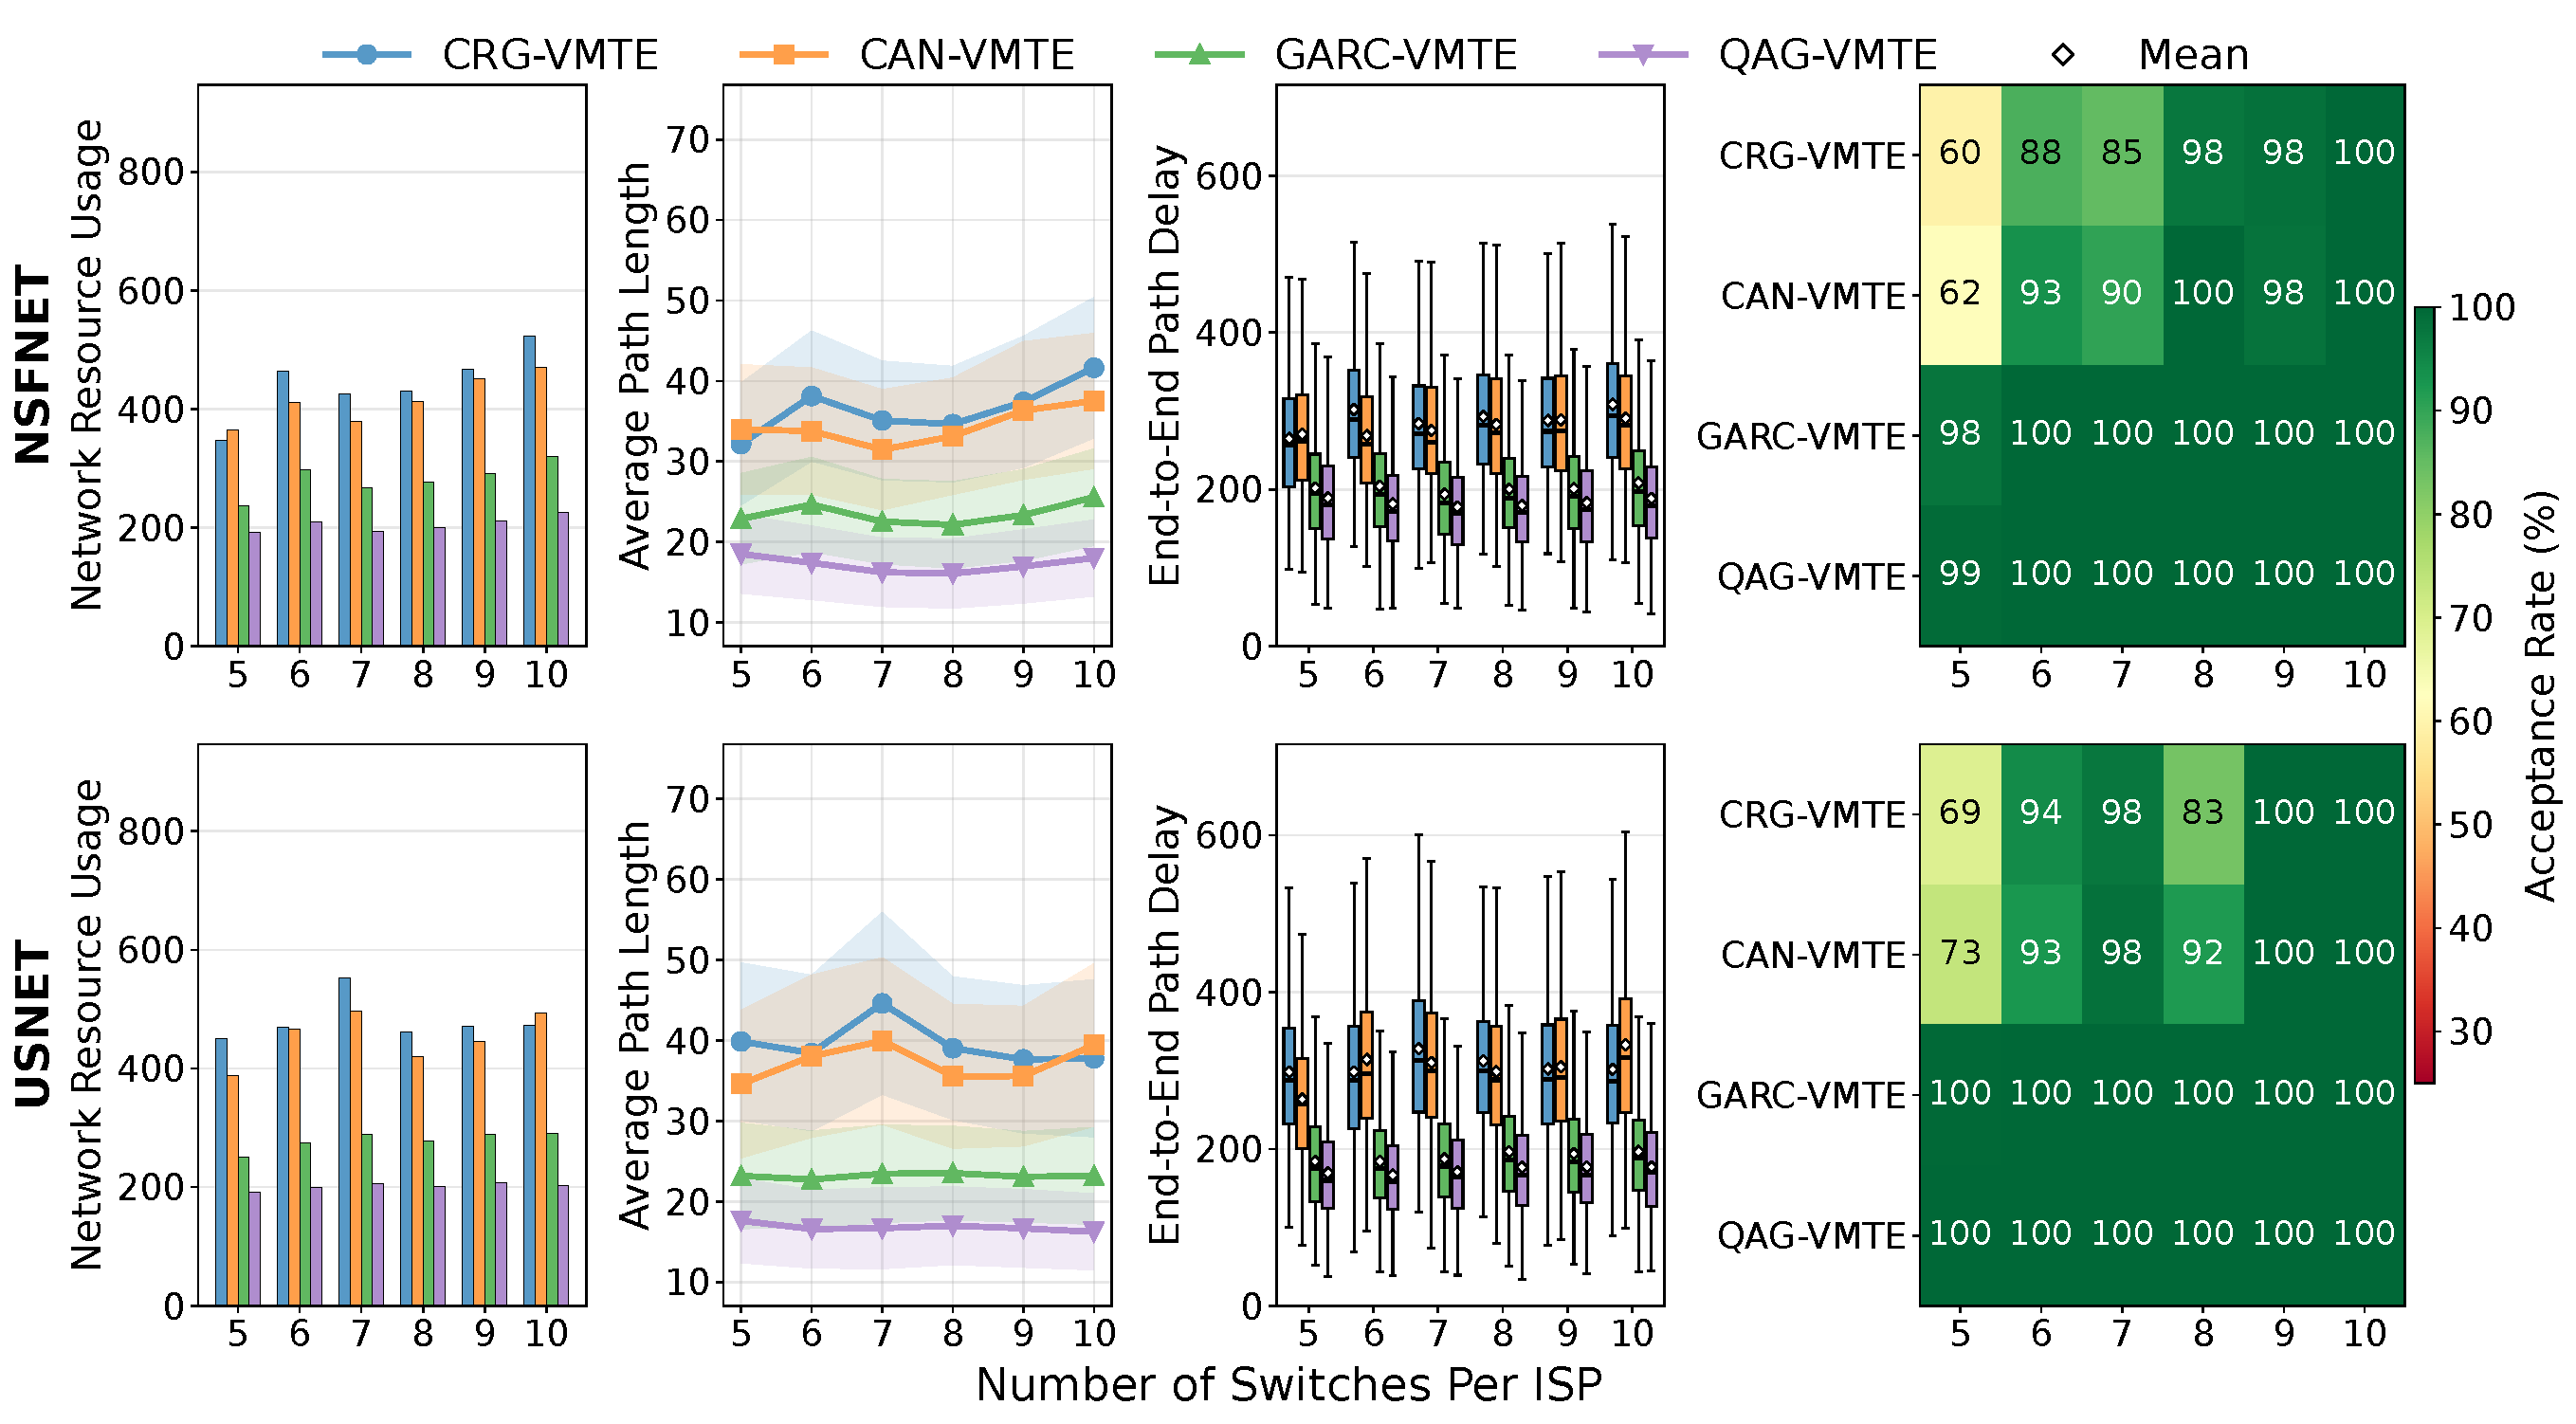
\includegraphics[width=\textwidth]{fig_results_ISP.pdf}
    \caption{ISP başına anahtar sayısına göre sonuçlar: üst satır NSFNET, alt satır USNET; soldan sağa ağ kaynak kullanımı, ortalama yol uzunluğu, uçtan uca yol gecikmesi ve kabul oranı (6--8 sanal düğüm, 10 veya 15 bant genişliği talebi).}
    \label{fig:results_isp}
\end{figure*}

\begin{table*}[!t]
\centering
\caption{ISP başına anahtar sayısı 5'ten 10'a çıkarıldığında uç değerler.}
\label{tab:isp}
\small
\begin{tabular}{lcccc}
\toprule
Algoritma & Ağ kaynak kullanımı & Ort. yol uzunluğu & Ort. uçtan uca gecikme & Kabul oranı (\%) \\
\midrule
\multicolumn{5}{l}{\textbf{NSFNET}} \\
CRG-VMTE & 347,4 $\rightarrow$ 522,4 & 32,2 $\rightarrow$ 41,6 & 264,9 $\rightarrow$ 308,4 & 59,5 $\rightarrow$ 100,0 \\
CAN-VMTE & 364,4 $\rightarrow$ 470,4 & 34,0 $\rightarrow$ 37,5 & 270,5 $\rightarrow$ 290,7 & 62,0 $\rightarrow$ 100,0 \\
GARC-VMTE & 236,2 $\rightarrow$ 320,6 & 22,9 $\rightarrow$ 25,6 & 201,9 $\rightarrow$ 208,1 & 97,7 $\rightarrow$ 100,0 \\
QAG-VMTE & 192,4 $\rightarrow$ 225,0 & 18,5 $\rightarrow$ 18,0 & 189,3 $\rightarrow$ 188,5 & 99,3 $\rightarrow$ 100,0 \\
\midrule
\multicolumn{5}{l}{\textbf{USNET}} \\
CRG-VMTE & 451,0 $\rightarrow$ 473,5 & 39,9 $\rightarrow$ 37,8 & 298,3 $\rightarrow$ 301,5 & 69,2 $\rightarrow$ 100,0 \\
CAN-VMTE & 387,3 $\rightarrow$ 494,2 & 34,6 $\rightarrow$ 39,4 & 263,5 $\rightarrow$ 332,7 & 73,3 $\rightarrow$ 100,0 \\
GARC-VMTE & 251,2 $\rightarrow$ 290,7 & 23,2 $\rightarrow$ 23,2 & 184,0 $\rightarrow$ 196,7 & 99,5 $\rightarrow$ 100,0 \\
QAG-VMTE & 191,7 $\rightarrow$ 202,7 & 17,6 $\rightarrow$ 16,2 & 169,4 $\rightarrow$ 177,0 & 99,8 $\rightarrow$ 100,0 \\
\bottomrule
\end{tabular}
\end{table*}

\paragraph{NSFNET.} En belirgin değişim kabul oranında, 5 anahtardan 6 anahtara geçişte görülmektedir: CRG-VMTE \%59,5'ten \%87,5'e, CAN-VMTE \%62,0'dan \%93,3'e yükselmektedir. Aynı geçişte alanların sunduğu pathlet sayısı 214'ten 808'e, yani yaklaşık 3,8 katına çıkmaktadır; 8 anahtardan sonra ise bu sayı 1377--1447 aralığında doygunluğa ulaşmakta, açgözlü yöntemlerin kabul oranı da \%97'nin üzerinde sabitlenmektedir. GA tabanlı yöntemler kaynak kısıtından çok daha az etkilenmektedir: 5 anahtarda bile GARC-VMTE \%97,7, QAG-VMTE \%99,3 kabul oranına ulaşmakta, 6 anahtardan itibaren ikisi de \%100'e çıkmaktadır. Açgözlü yöntemlerin eğrisi tekdüze değildir; 7 anahtarda CRG-VMTE 2,2, CAN-VMTE 3,2 puan gerilemekte, CAN-VMTE 9 anahtarda yeniden 1,7 puan kaybetmektedir.

Ağ kaynak kullanımında, ortak istek sayısı 5 anahtarda 314 ile sınırlı olduğundan ölçeklenme eğilimini 6 anahtardan itibaren okumak daha sağlıklıdır. 6 anahtardan 10 anahtara kullanım CRG-VMTE'de \%12,8, CAN-VMTE'de \%14,4, GARC-VMTE'de \%8,0, QAG-VMTE'de \%7,0 artmaktadır; dolayısıyla GA tabanlı yöntemler büyüyen ağda daha yavaş bozulmaktadır. QAG-VMTE, CRG-VMTE'ye göre \%44,6--56,9, CAN-VMTE'ye göre \%47,2--53,2, GARC-VMTE'ye göre \%18,6--29,8 daha az kaynak kullanmaktadır; bu fark 10 anahtarda en yüksek düzeye ya da ona yakın bir düzeye ulaşmaktadır. CAN-VMTE'nin CRG-VMTE'ye üstünlüğü ise kararsızdır: 6 anahtarda \%11,2 avantaj sağlarken 5 anahtarda \%4,9 daha fazla kaynak tüketmektedir.

Yol uzunluğu kaynak kullanımıyla aynı örüntüyü izlemektedir. QAG-VMTE'nin yol uzunluğu 5 anahtarda 18,5 iken 8 anahtarda 16,1'e inmekte, 10 anahtarda 18,0'a dönmektedir. GARC-VMTE 22,1--25,6, CAN-VMTE 31,5--37,5, CRG-VMTE ise 32,2--41,6 aralığındadır. Anahtar sayısı arttıkça alternatif yolların çoğalmasına rağmen yol uzunluğunun azalmaması dikkat çekicidir; 8 anahtardan sonra alan içi güzergâhların uzamasının bu kazanımı dengelediği düşünülmektedir.

Gecikmede QAG-VMTE 177,5--189,3, GARC-VMTE 194,0--208,1 aralığında kalırken CRG-VMTE 264,9--308,4, CAN-VMTE 268,7--290,7 aralığındadır. QAG-VMTE, 6 anahtardan itibaren CRG-VMTE'den \%36,4--39,8 daha düşük gecikme sağlamaktadır. CRG-VMTE'nin 5 anahtardaki düşük gecikmesi (264,9) gerçek bir üstünlük olarak okunmamalıdır: bu noktada yalnızca isteklerin \%59,5'i kabul edilmiş ve kabul edilen isteklerin ortalama bant genişliği talebi 11,2'ye gerilemiştir (\%100 kabulde 12,5). Kabul oranı 6 anahtarda yükselince gecikme de \%14,0 artarak 301,8'e çıkmaktadır.

\paragraph{USNET.} Kabul oranında 5 anahtardaki düşüklük burada da görülmektedir (CRG-VMTE \%69,2; CAN-VMTE \%73,3), ancak NSFNET'e göre daha ılımlıdır; bu durum alan başına pathlet sayısının daha yüksek olmasıyla (USNET'te 23,3; NSFNET'te 15,3) uyumludur. En dikkat çekici sonuç 8 anahtarda ortaya çıkmaktadır: 7 anahtarda \%97,5 olan CRG-VMTE kabul oranı \%83,2'ye, \%98,5 olan CAN-VMTE kabul oranı \%91,8'e düşmekte; GARC-VMTE ise yalnızca 0,2 puan kaybetmekte, QAG-VMTE \%100'de kalmaktadır. 9 anahtardan itibaren dört yöntem de \%100'e ulaşmaktadır. Bu kırılma bir eşik etkisine benzemektedir ve her anahtar ölçeğinde ayrı iç topoloji örnekleri kullanıldığından, ilgili örneklerdeki darboğazlardan kaynaklanması muhtemeldir. Bu darboğazları açgözlü yöntemlerin aşamaması, GA tabanlı yöntemlerin ise kolayca aşması, arama derinliğinin dayanıklılığa katkı sağladığını düşündürmektedir.

Ağ kaynak kullanımında USNET'in ölçeklenme davranışı NSFNET'ten farklıdır: 6 anahtardan 10 anahtara artış CRG-VMTE'de yalnızca \%0,9, QAG-VMTE'de \%1,4, CAN-VMTE ve GARC-VMTE'de yaklaşık \%6'dır. CRG-VMTE'nin kullanımı 451,0--553,3 aralığında dalgalanıp 7 anahtarda belirgin bir tepe yaparken QAG-VMTE 191,7--208,1 gibi dar bir bantta kalmaktadır. QAG-VMTE, CRG-VMTE'ye göre \%55,9--62,8, CAN-VMTE'ye göre \%50,5--59,0, GARC-VMTE'ye göre \%23,7--30,3 daha az kaynak kullanmaktadır. Yol uzunluğu da benzer biçimde GARC-VMTE'de (22,7--23,5) ve QAG-VMTE'de (16,2--17,6) neredeyse düzdür. CRG-VMTE ise 37,7--44,6 aralığında dalgalanmaktadır.

Gecikmede GA tabanlı yöntemler anahtar sayısıyla hafifçe yükselmektedir (GARC-VMTE 184,0'dan 196,7'ye, QAG-VMTE 169,4'ten 177,0'a). QAG-VMTE, CRG-VMTE'den \%41,3--47,9, GARC-VMTE'den \%7,9--10,1 daha düşük gecikme sağlamaktadır. CAN-VMTE bu ağda belirgin biçimde kararsızdır: 5 anahtarda CRG-VMTE'den \%11,6 düşük gecikme verirken 10 anahtarda \%10,3 daha yüksek gecikme vermekte ve kaynak kullanımında da \%4,4 geride kalmaktadır. Başka bir deyişle merkezilik bilgisi, tek başına tutarlı bir kazanç garantisi vermemektedir.

\paragraph{Ortak bulgular.} İki ağda da (i)~5 anahtarlı ölçek açgözlü yöntemler için kaynak bakımından kritik eşiktir ve kabul oranı anahtar sayısıyla tekdüze olmayan biçimde iyileşmektedir; (ii)~GA tabanlı yöntemler 6 anahtardan itibaren fiilen doygun kabul oranına ulaşmaktadır; (iii)~QAG-VMTE metriklerin tamamında en iyi sonucu vermektedir; (iv)~anahtar sayısının artması yol uzunluğunu ve gecikmeyi belirgin biçimde kısaltmamakta, asıl kazanım kabul oranında görülmektedir. Temel fark, kırılma noktasının konumudur (NSFNET'te 7, USNET'te 8 anahtar) ve USNET'te açgözlü yöntemlerle GA tabanlı yöntemler arasındaki farkın daha büyük olmasıdır.

\subsection{Bant Genişliği Talebinin Etkisi}

Bu alt bölümde bant genişliği talebi 5'ten 25'e çıkarılmış, sonuçlar 6, 7 ve 8 anahtarlı ölçekler üzerinden birleştirilmiştir (nokta başına 1800 istek). Sonuçlar Şekil~\ref{fig:results_vbw} ve Tablo~\ref{tab:vbw}'de verilmiştir. Bu parametre, algoritmaların kapasite baskısına verdiği tepkiyi en açık gösteren parametredir.

\begin{figure*}[!t]
    \centering
    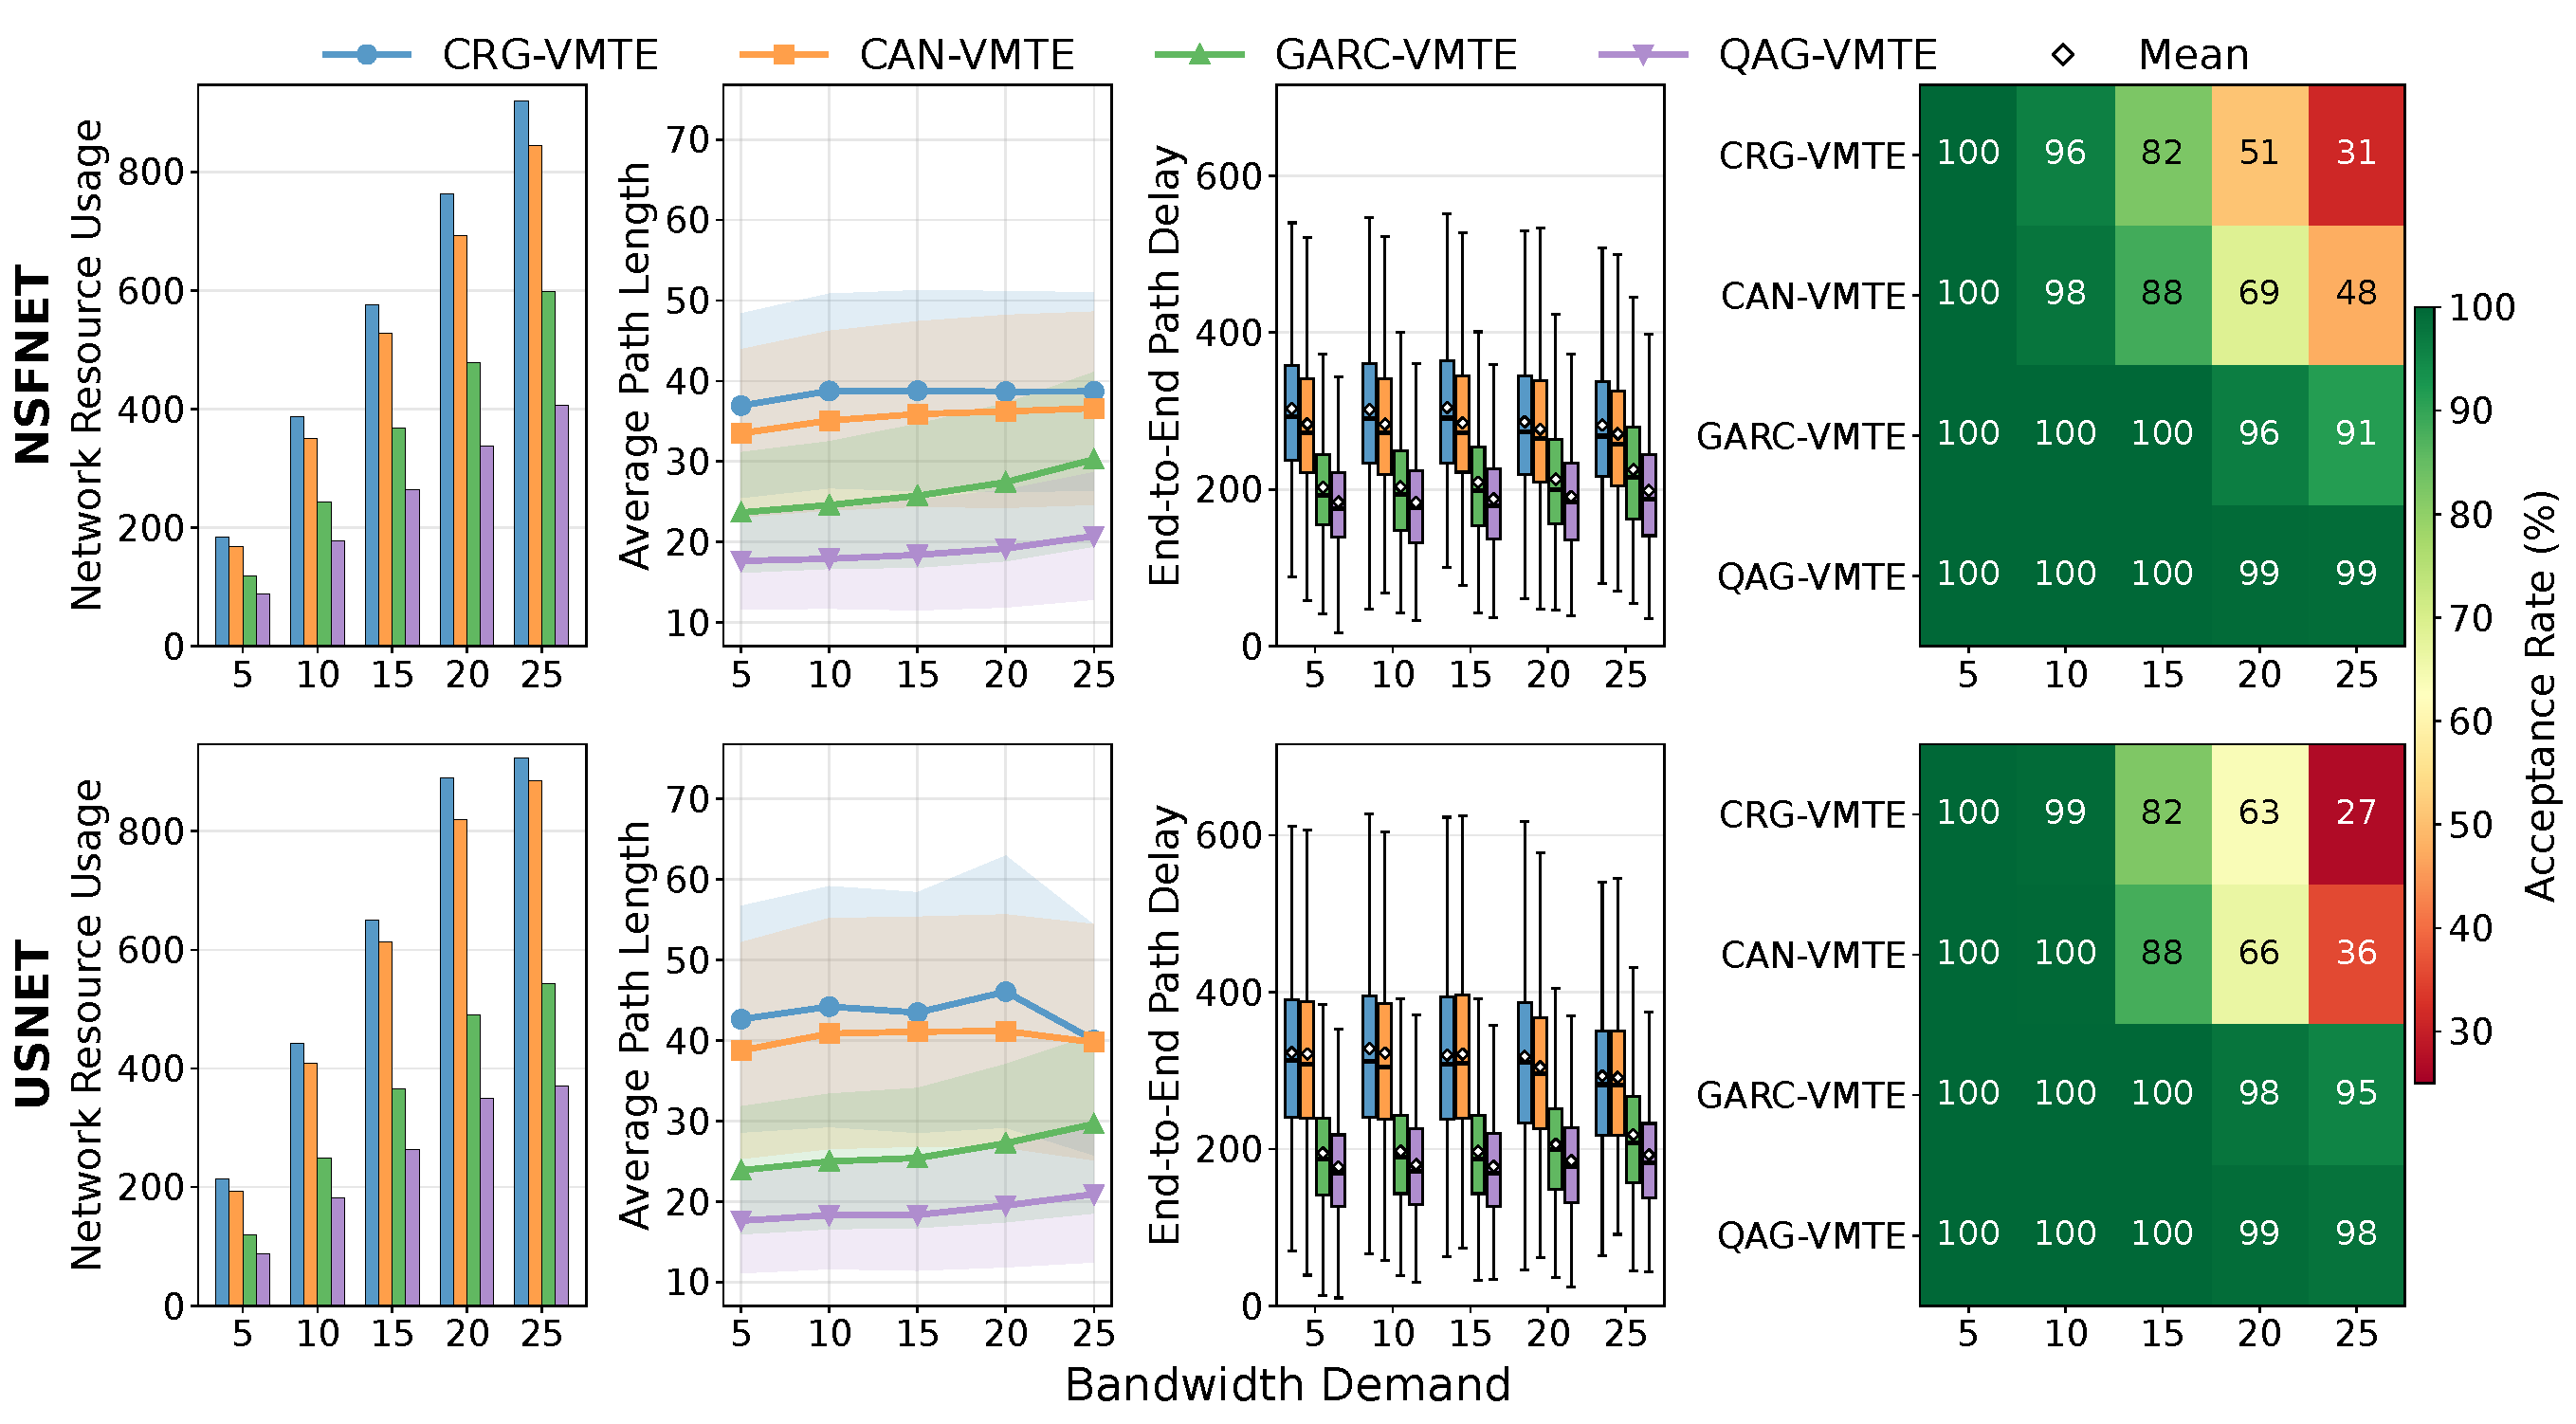
\includegraphics[width=\textwidth]{fig_results_VBW.pdf}
    \caption{Bant genişliği talebine göre sonuçlar: üst satır NSFNET, alt satır USNET; soldan sağa ağ kaynak kullanımı, ortalama yol uzunluğu, uçtan uca yol gecikmesi ve kabul oranı (6, 7 ve 8 anahtarlı ölçekler birleştirilmiştir).}
    \label{fig:results_vbw}
\end{figure*}

\begin{table*}[!t]
\centering
\caption{Bant genişliği talebi 5'ten 25'e çıkarıldığında uç değerler.}
\label{tab:vbw}
\small
\begin{tabular}{lcccc}
\toprule
Algoritma & Ağ kaynak kullanımı & Ort. yol uzunluğu & Ort. uçtan uca gecikme & Kabul oranı (\%) \\
\midrule
\multicolumn{5}{l}{\textbf{NSFNET}} \\
CRG-VMTE & 184,7 $\rightarrow$ 920,0 & 36,9 $\rightarrow$ 38,7 & 303,0 $\rightarrow$ 282,0 & 99,9 $\rightarrow$ 31,3 \\
CAN-VMTE & 167,5 $\rightarrow$ 844,8 & 33,5 $\rightarrow$ 36,6 & 283,5 $\rightarrow$ 270,9 & 100,0 $\rightarrow$ 47,6 \\
GARC-VMTE & 118,3 $\rightarrow$ 598,7 & 23,7 $\rightarrow$ 30,3 & 202,7 $\rightarrow$ 225,2 & 100,0 $\rightarrow$ 91,4 \\
QAG-VMTE & 88,3 $\rightarrow$ 406,8 & 17,7 $\rightarrow$ 20,7 & 184,0 $\rightarrow$ 198,4 & 100,0 $\rightarrow$ 99,1 \\
\midrule
\multicolumn{5}{l}{\textbf{USNET}} \\
CRG-VMTE & 213,2 $\rightarrow$ 923,7 & 42,6 $\rightarrow$ 40,0 & 322,8 $\rightarrow$ 293,2 & 100,0 $\rightarrow$ 26,8 \\
CAN-VMTE & 193,8 $\rightarrow$ 885,6 & 38,8 $\rightarrow$ 39,8 & 321,3 $\rightarrow$ 291,1 & 100,0 $\rightarrow$ 35,7 \\
GARC-VMTE & 119,4 $\rightarrow$ 543,4 & 23,9 $\rightarrow$ 29,6 & 194,9 $\rightarrow$ 218,1 & 100,0 $\rightarrow$ 95,3 \\
QAG-VMTE & 88,1 $\rightarrow$ 371,2 & 17,6 $\rightarrow$ 20,9 & 177,0 $\rightarrow$ 192,6 & 100,0 $\rightarrow$ 98,2 \\
\bottomrule
\end{tabular}
\end{table*}

\paragraph{NSFNET.} 10'a kadar olan taleplerde tüm yöntemlerin kabul oranı \%96'nın üzerindedir; ayrışma 15 talebinde başlamaktadır (CRG-VMTE \%82,3; CAN-VMTE \%88,5; GA tabanlı yöntemler \%100). En sert kırılma 15'ten 20'ye geçiştedir: CRG-VMTE 31,5, CAN-VMTE 19,7 puan kaybetmektedir. 25 talebinde CRG-VMTE \%31,3 ve CAN-VMTE \%47,6'ya inerken GARC-VMTE \%91,4'te, QAG-VMTE \%99,1'de kalmaktadır; QAG-VMTE burada CRG-VMTE'nin 3,2 katı kabul oranı sunmaktadır. İki GA arasındaki en büyük fark da bu noktadadır (7,7 puan). Q-öğrenmeli seçimin katkısı, kapasite baskısı arttıkça görünür hale gelmektedir.

Ağ kaynak kullanımı talep ile neredeyse doğrusal artmaktadır. Talep 5 katına çıktığında kuramsal artış \%400 iken CRG-VMTE'de \%398,1, CAN-VMTE'de \%404,3, GARC-VMTE'de \%405,9, QAG-VMTE'de \%360,9 artış ölçülmüştür. Kaynak kullanımı, talep ile atlama sayısının çarpımı olduğundan bu beklenen bir sonuçtur ve metrikler arasındaki doğrudan bağı göstermektedir. QAG-VMTE'nin farkı talep arttıkça büyümektedir: CRG-VMTE'ye göre \%52,2'den \%55,8'e, GARC-VMTE'ye göre \%25,4'ten \%32,0'a çıkmaktadır. CAN-VMTE'nin CRG-VMTE'ye avantajı \%8,2--9,4 ile sabit kalmaktadır.

Yol uzunluğu ve gecikme, algoritma ailelerini ters yönlere ayırmaktadır. GA tabanlı yöntemlerde yol uzunluğu artmaktadır (GARC-VMTE 23,7'den 30,3'e, +\%27,9; QAG-VMTE 17,7'den 20,7'ye, +\%17,5) ve gecikme de yükselmektedir (GARC-VMTE +\%11,1; QAG-VMTE +\%7,8). Açgözlü yöntemlerde ise yol uzunluğu neredeyse sabittir (CRG-VMTE +\%4,8; CAN-VMTE +\%9,3) ve gecikme düşmektedir (CRG-VMTE $-$\%6,9; CAN-VMTE $-$\%4,4). Bu düşüş bir iyileşme değildir: açgözlü yöntemler zor istekleri reddettiği için, 25 talebinde kabul ettikleri isteklerin ortalama sanal düğüm sayısı 7,5'ten 6,8--7,0 düzeyine gerilemektedir. GA tabanlı yöntemler ise aynı istekleri daha uzun yollar bularak kabul etmektedir. Yalnızca ortak isteklere bakıldığında bu etki büyük ölçüde ortadan kalkmaktadır: 25 talebinde QAG-VMTE'nin gecikme avantajı, kendi kabul ettiği isteklerde \%29,6 iken ortak isteklerde \%36,4'tür. Benzer şekilde yol uzunluğu avantajı \%46,4'ten \%55,8'e çıkmaktadır.

\paragraph{USNET.} Kabul oranı örüntüsü benzerdir, ancak kırılma daha geç ve daha serttir: 20 talebinde CRG-VMTE hâlâ \%63,4 kabul oranına sahipken (NSFNET'te \%50,8) 25 talebinde 36,6 puan kaybederek \%26,8'e düşmektedir; CAN-VMTE 30,6 puan kaybederek \%35,7'ye inmektedir. GARC-VMTE \%95,3 ve QAG-VMTE \%98,2 ile yüksek kalmakta, QAG-VMTE burada CRG-VMTE'nin 3,7 katına ulaşmaktadır. İki GA arasındaki fark 2,8 puanla NSFNET'tekinden küçüktür.

Ağ kaynak kullanımında bu ağa özgü dikkat çekici bir sonuç, 20'den 25'e geçişte artışın beklenen \%25'in çok altında kalmasıdır (CRG-VMTE +\%3,7; QAG-VMTE +\%6,2; CAN-VMTE +\%8,0; GARC-VMTE +\%11,0). Bu, kapasite kazancı değil, örneklem etkisidir: ortak istek sayısı 892'den 232'ye, bu isteklerin ortalama sanal düğüm sayısı 7,05'ten 6,06'ya düşmektedir. NSFNET'te ortak istek kaybı daha sınırlı olduğundan (773'ten 393'e) artış \%20--25 düzeyinde kalmaktadır. Dolayısıyla USNET'in 25 talebindeki kaynak değerleri daha küçük isteklerin ortalaması olarak yorumlanmalıdır. Algoritmalar arası farklar ise bu etkiden görece bağımsızdır: QAG-VMTE, CRG-VMTE'ye göre \%58,7--60,8, CAN-VMTE'ye göre \%54,5--58,1, GARC-VMTE'ye göre \%26,2--31,7 daha az kaynak kullanmaktadır.

Yol uzunluğu ve gecikmede NSFNET'teki ayrışma tekrarlanmaktadır. GARC-VMTE +\%24,1 ve QAG-VMTE +\%18,6 yol uzunluğu artışı gösterirken CRG-VMTE $-$\%6,1 azalmakta, CAN-VMTE +\%2,7 ile yatay kalmaktadır. Gecikme GARC-VMTE'de +\%11,9, QAG-VMTE'de +\%8,8 artarken CRG-VMTE'de $-$\%9,2, CAN-VMTE'de $-$\%9,4 azalmaktadır. QAG-VMTE'nin 25 talebindeki gecikme avantajı kendi kabul ettiği isteklerde \%34,3, ortak isteklerde \%43,7'dir. CAN-VMTE ile CRG-VMTE'nin gecikmesi bu ağda neredeyse aynıdır (fark en fazla \%4,2).

\paragraph{Ortak bulgular.} İki ağda da talep artışı, açgözlü yöntemlerde istekleri reddederek, GA tabanlı yöntemlerde yolları uzatarak karşılanmaktadır. Talep ile yol uzunluğu korelasyonunun GA tabanlı yöntemlerde (0,15--0,24) açgözlü yöntemlerden (0,02--0,09) yüksek olması bu farkı doğrulamaktadır. Her iki ağda sıralama genel olarak QAG-VMTE, GARC-VMTE, CAN-VMTE, CRG-VMTE şeklindedir; tek istisna, CAN-VMTE ile CRG-VMTE'nin USNET'te gecikme bakımından ayrışmamasıdır. Bu bölümün temel sonucu, QAG-VMTE'nin kabul oranı ile kaynak verimliliğini aynı anda koruyabilmesidir; artan kabul oranı daha yüksek kaynak kullanımı pahasına elde edilmemektedir.

\subsection{Sanal Düğüm Sayısının Etkisi}

Bu alt bölümde istek başına sanal düğüm sayısı 5'ten 10'a çıkarılmış, sonuçlar 6, 7 ve 8 anahtarlı ölçekler üzerinden birleştirilmiştir (nokta başına 1500 istek). Sonuçlar Şekil~\ref{fig:results_vnode} ve Tablo~\ref{tab:vnode}'de verilmiştir.

\begin{figure*}[!t]
    \centering
    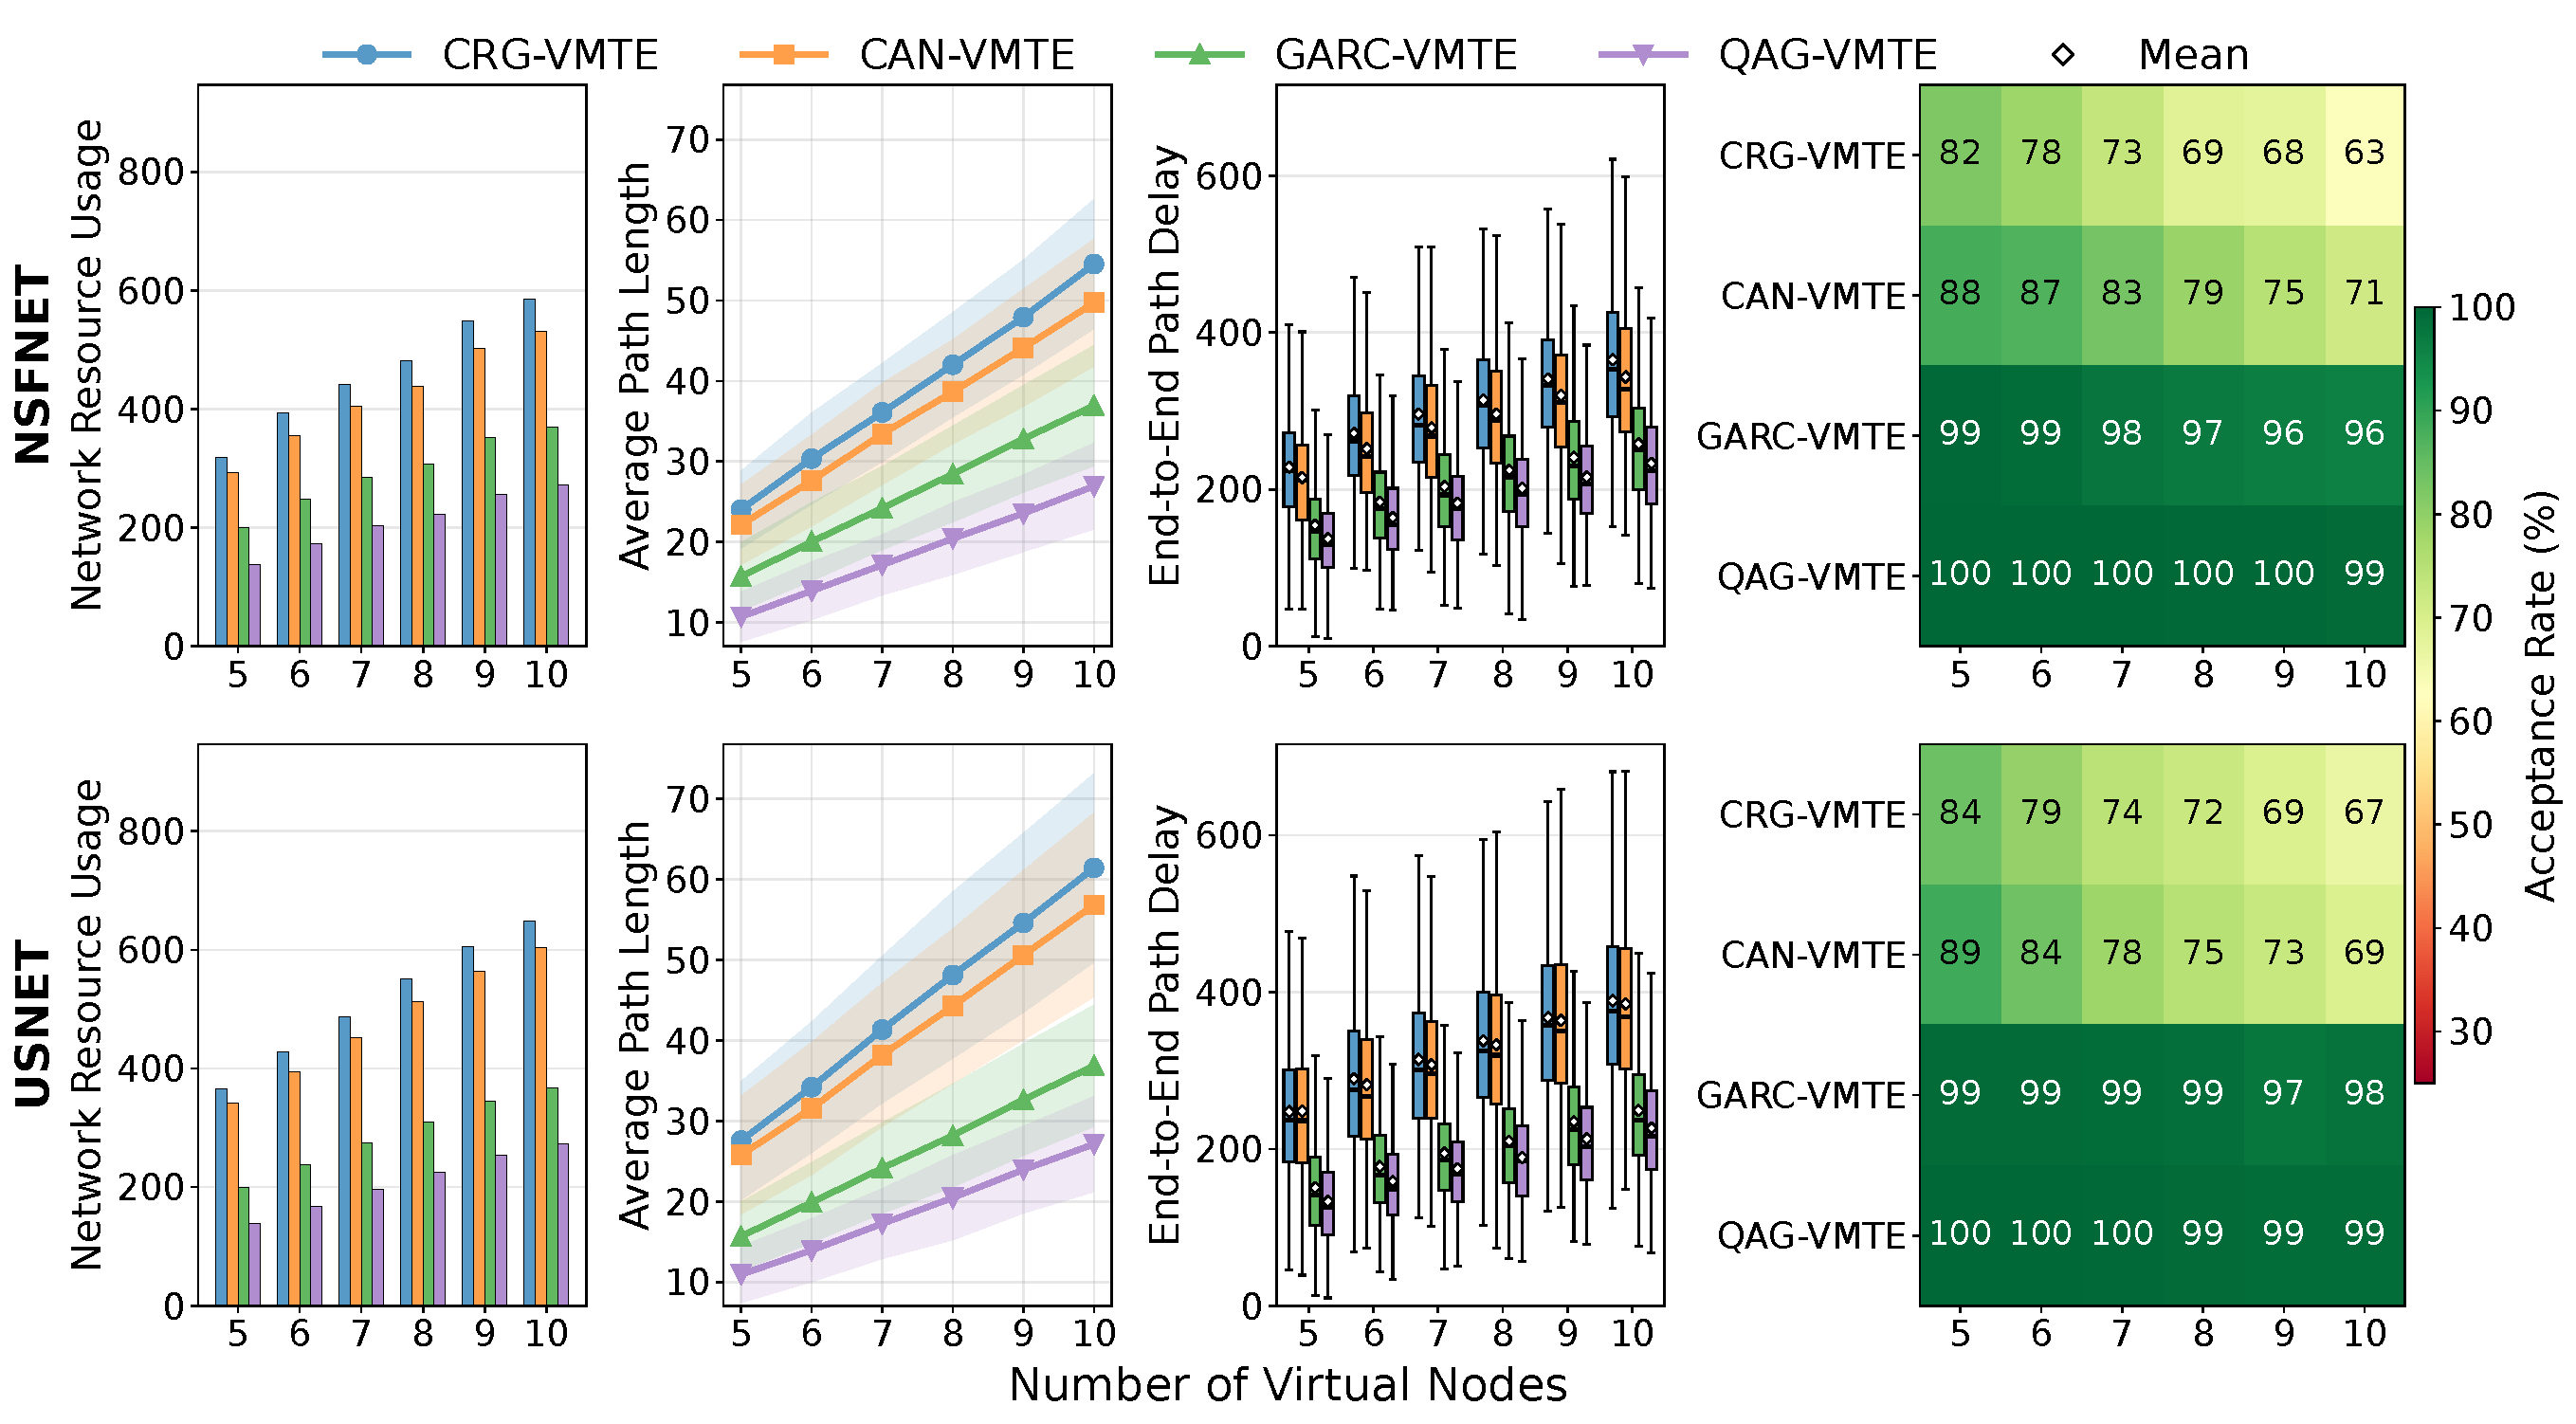
\includegraphics[width=\textwidth]{fig_results_VNode.pdf}
    \caption{Sanal düğüm sayısına göre sonuçlar: üst satır NSFNET, alt satır USNET; soldan sağa ağ kaynak kullanımı, ortalama yol uzunluğu, uçtan uca yol gecikmesi ve kabul oranı (6, 7 ve 8 anahtarlı ölçekler birleştirilmiştir).}
    \label{fig:results_vnode}
\end{figure*}

\begin{table*}[!t]
\centering
\caption{Sanal düğüm sayısı 5'ten 10'a çıkarıldığında uç değerler.}
\label{tab:vnode}
\small
\begin{tabular}{lcccc}
\toprule
Algoritma & Ağ kaynak kullanımı & Ort. yol uzunluğu & Ort. uçtan uca gecikme & Kabul oranı (\%) \\
\midrule
\multicolumn{5}{l}{\textbf{NSFNET}} \\
CRG-VMTE & 318,1 $\rightarrow$ 584,7 & 24,0 $\rightarrow$ 54,5 & 228,6 $\rightarrow$ 365,4 & 81,9 $\rightarrow$ 62,9 \\
CAN-VMTE & 292,1 $\rightarrow$ 531,5 & 22,1 $\rightarrow$ 49,7 & 215,3 $\rightarrow$ 343,5 & 88,1 $\rightarrow$ 71,4 \\
GARC-VMTE & 200,2 $\rightarrow$ 369,8 & 15,7 $\rightarrow$ 36,9 & 154,4 $\rightarrow$ 258,0 & 99,5 $\rightarrow$ 96,0 \\
QAG-VMTE & 137,1 $\rightarrow$ 272,4 & 10,7 $\rightarrow$ 26,9 & 137,1 $\rightarrow$ 233,2 & 99,9 $\rightarrow$ 99,3 \\
\midrule
\multicolumn{5}{l}{\textbf{USNET}} \\
CRG-VMTE & 365,0 $\rightarrow$ 649,0 & 27,6 $\rightarrow$ 61,4 & 247,5 $\rightarrow$ 389,1 & 84,0 $\rightarrow$ 66,5 \\
CAN-VMTE & 342,3 $\rightarrow$ 604,2 & 25,8 $\rightarrow$ 56,8 & 248,1 $\rightarrow$ 385,0 & 88,7 $\rightarrow$ 69,3 \\
GARC-VMTE & 199,1 $\rightarrow$ 367,1 & 15,7 $\rightarrow$ 36,9 & 150,7 $\rightarrow$ 248,9 & 99,3 $\rightarrow$ 98,1 \\
QAG-VMTE & 138,1 $\rightarrow$ 272,4 & 10,9 $\rightarrow$ 27,1 & 133,0 $\rightarrow$ 226,6 & 99,8 $\rightarrow$ 98,9 \\
\bottomrule
\end{tabular}
\end{table*}

\paragraph{NSFNET.} Sanal düğüm sayısı arttıkça kabul oranı açgözlü yöntemlerde kademeli olarak düşmektedir: CRG-VMTE \%81,9'dan \%62,9'a (18,9 puan), CAN-VMTE \%88,1'den \%71,4'e (16,7 puan). GARC-VMTE \%99,5'ten \%96,0'a inmekte, QAG-VMTE ise \%99,3'ün altına düşmemektedir. Bu nedenle QAG-VMTE'nin CRG-VMTE'ye göre göreli üstünlüğü \%22,0'dan \%57,7'ye yükselmektedir. Bant genişliği parametresindeki sert kırılmanın aksine bu düşüş daha düzenlidir. Sanal düğüm sayısının etkisi bant genişliği talebiyle birlikte güçlenmektedir: 5 talebinde tüm bileşimler yaklaşık \%100 kabul edilirken, 25 talebinde CRG-VMTE'nin kabul oranı 5 sanal düğümde \%50'den 10 sanal düğümde \%14'e düşmekte, QAG-VMTE'ninki ise yaklaşık \%98'in altına inmemektedir.

Yol uzunluğu tüm yöntemlerde en güçlü artışı bu parametrede göstermektedir: CRG-VMTE +\%126,8, CAN-VMTE +\%124,6, GARC-VMTE +\%135,2, QAG-VMTE +\%151,5. Bu artış, sanal bağlantı sayısının 4'ten 9'a çıkmasından (+\%125) kaynaklanmaktadır. Sanal bağlantı başına atlama sayısı hesaplandığında CRG-VMTE'nin 6,0--6,1, CAN-VMTE'nin 5,5--5,6 ile sabit kaldığı görülmektedir. GARC-VMTE 3,9'dan 4,1'e, QAG-VMTE 2,7'den 3,0'a hafifçe yükselmektedir. Yani QAG-VMTE'nin yüzde olarak en hızlı artışı gösteren yöntem olması bir zayıflık değil, büyük ölçüde başlangıç değerinin çok düşük olmasının sonucudur. Mutlak olarak QAG-VMTE'nin yol uzunluğu 10,7'den 26,9'a (+16,2), CRG-VMTE'ninki 24,0'dan 54,5'e (+30,5) çıkmaktadır.

Ağ kaynak kullanımı QAG-VMTE'de +\%98,7, GARC-VMTE'de +\%84,7, CRG-VMTE'de +\%83,8, CAN-VMTE'de +\%82,0 artmaktadır. Mutlak artış ise QAG-VMTE'de 135,3, CRG-VMTE'de 266,6'dır. Kaynak kullanımının yol uzunluğundan daha yavaş artmasının nedeni ortak istek kümesinin bileşimidir: sanal düğüm arttıkça ortak kümedeki ortalama bant genişliği talebi 12,97'den 10,60'a gerilemektedir. QAG-VMTE, CRG-VMTE'ye göre \%53,4--56,9, CAN-VMTE'ye göre \%48,8--53,1, GARC-VMTE'ye göre \%26,3--31,5 daha az kaynak kullanmaktadır.

Gecikme, yol uzunluğuna göre belirgin biçimde daha yavaş artmaktadır (CRG-VMTE +\%59,8; CAN-VMTE +\%59,6; GARC-VMTE +\%67,1; QAG-VMTE +\%70,1). Bunun nedeni, yol uzunluğu tüm sanal bağlantıların toplamı iken gecikmenin en uzun uçtan uca yolla belirlenmesidir. QAG-VMTE, CRG-VMTE'den \%35,8--40,0, GARC-VMTE'den \%9,6--11,2 daha düşük gecikme sağlamaktadır.

\paragraph{USNET.} Kabul oranında CRG-VMTE \%84,0'tan \%66,5'e (17,5 puan), CAN-VMTE \%88,7'den \%69,3'e (19,4 puan) düşmekte; GARC-VMTE ve QAG-VMTE sırasıyla \%97,4 ve \%98,9'un altına inmemektedir. NSFNET'ten önemli bir farkla, CAN-VMTE'nin CRG-VMTE'ye sağladığı kabul oranı avantajı yalnızca 2,8--4,7 puandır (NSFNET'te 6,2--10,3 puan). Yol uzunluğu CRG-VMTE'de +\%122,9, CAN-VMTE'de +\%120,5, GARC-VMTE'de +\%135,2, QAG-VMTE'de +\%147,9 artmaktadır. Sanal bağlantı başına atlama sayısı CRG-VMTE'de 6,8--6,9, CAN-VMTE'de 6,3--6,5, GARC-VMTE'de 3,9--4,1, QAG-VMTE'de 2,7--3,0'dır.

Ağ kaynak kullanımı QAG-VMTE'de +\%97,2 (mutlak 134,3), GARC-VMTE'de +\%84,4, CRG-VMTE'de +\%77,8 (mutlak 283,9), CAN-VMTE'de +\%76,5 artmaktadır. QAG-VMTE, CRG-VMTE'ye göre \%58,0--62,2, CAN-VMTE'ye göre \%54,9--59,7, GARC-VMTE'ye göre \%25,8--30,6 daha az kaynak kullanmaktadır. Gecikme QAG-VMTE'de 133,0'dan 226,6'ya, CRG-VMTE'de 247,5'ten 389,1'e çıkmaktadır. QAG-VMTE, CRG-VMTE'den \%41,8--46,3, GARC-VMTE'den \%9,0--11,7 daha düşük gecikme sağlamaktadır. Dikkat çekici bir başka sonuç, CAN-VMTE'nin bu ağda gecikme bakımından CRG-VMTE'den neredeyse hiç ayrışmamasıdır (fark en fazla \%2,7; NSFNET'te \%5,7--7,2).

\paragraph{Ortak bulgular.} İki ağda da sanal düğüm sayısı, yol uzunluğu ve gecikme üzerinde en güçlü parametredir (korelasyon yol uzunluğu için 0,75--0,85, gecikme için 0,42--0,46); kaynak kullanımında ise bant genişliği talebi daha baskındır (0,76--0,82). Yöntemlerin sanal bağlantı başına atlama sayısı istek boyutundan büyük ölçüde bağımsızdır; bu da istek büyüdükçe yöntemlerin yol kalitesinin korunduğunu göstermektedir. QAG-VMTE'nin göreli farkı istek büyüdükçe bir miktar daralsa da (örneğin kaynak kullanımında NSFNET'te \%56,9'dan \%53,4'e, USNET'te \%62,2'den \%58,0'a) mutlak fark büyümektedir. Üstelik kabul oranı açgözlü yöntemlerde düşerken QAG-VMTE'de sabit kaldığından, büyük isteklerdeki gerçek üstünlük bu oranların gösterdiğinden daha büyüktür.

\subsection*{Bulguların Genel Değerlendirmesi}

\paragraph{Algoritmalar arası genel tablo.} Tüm parametre uzayında (ağ başına 18.000 çözüm) kabul oranı NSFNET'te CRG-VMTE için \%73,5, CAN-VMTE için \%78,3, GARC-VMTE için \%96,2, QAG-VMTE için \%98,5; USNET'te sırasıyla \%78,0, \%79,9, \%97,4 ve \%98,7'dir. 6--8 anahtarlı ölçeklerde QAG-VMTE'nin kabul edip CRG-VMTE'nin reddettiği isteklerin oranı NSFNET'te \%27,6, USNET'te \%25,1'dir. Dört yöntemin de kabul ettiği aynı istekler üzerinde eşleştirilmiş karşılaştırma yapıldığında (NSFNET'te 6043, USNET'te 6065 istek), QAG-VMTE ortak isteklerin neredeyse tamamında CRG-VMTE'den ve CAN-VMTE'den daha az kaynak kullanmakta, GARC-VMTE'yi ise isteklerin \%99,5'inden fazlasında geçmektedir. Gecikmede QAG-VMTE, CRG-VMTE'yi isteklerin yaklaşık \%97'sinde, GARC-VMTE'yi yaklaşık \%84--85'inde geçmektedir. Buna karşın CAN-VMTE, CRG-VMTE'den daha az kaynağı NSFNET'te isteklerin \%65,1'inde, USNET'te \%60,8'inde kullanmakta, gecikmedeki üstünlüğü ise USNET'te \%52,0 ile rastlantı düzeyine yaklaşmaktadır. Ayrıca kutu grafiklerinde görüldüğü üzere QAG-VMTE'nin gecikme dağılımı daha dardır: çeyrekler açıklığı QAG-VMTE'de 93--94 iken CRG-VMTE'de NSFNET'te 126, USNET'te 152'dir.

\paragraph{Metrikler arası ilişki.} Ağ kaynak kullanımı, bant genişliği talebi ile atlama sayısının çarpımı olduğundan bir istek için yol uzunluğunun doğrudan bir ölçeklenmiş halidir; bu yüzden iki metriğin göreli farkları neredeyse aynıdır. Gecikme ile yol uzunluğu arasındaki korelasyon ise 0,58--0,66 ile yalnızca orta-güçlü düzeydedir ve iki metrikteki kazançlar birbirine eşit değildir. Ortak isteklerde QAG-VMTE, GARC-VMTE'ye göre atlama sayısını yaklaşık \%27 azaltırken gecikmeyi yalnızca \%9,5--9,8 azaltmaktadır. Bu farkın nedeni kaydedilen yollarda görülmektedir: QAG-VMTE ile GARC-VMTE'nin alanlar arası geçiş sayıları hemen hemen aynıdır (NSFNET'te 8,45 ve 8,71; USNET'te 8,32 ve 8,58), oysa toplam atlama sayıları belirgin biçimde farklıdır (NSFNET'te 18,8 ve 26,3; USNET'te 18,9 ve 26,2). Yani QAG-VMTE'nin kazancının büyük bölümü alan içi atlamalardan gelmektedir. Alanlar arası bir bağlantının gecikmesi alan içi bir bağlantının yaklaşık 5,5 katı olduğundan bu azalma gecikmeye sınırlı yansımaktadır. Buna karşılık GA tabanlı yöntemler açgözlü yöntemlere göre alanlar arası geçişleri de azaltmaktadır: CRG-VMTE'den GARC-VMTE'ye geçiş sayısı NSFNET'te 13,24'ten 8,71'e ($-$\%34,2), USNET'te 14,49'dan 8,58'e ($-$\%40,8) düşmekte, gecikme de ortak isteklerde buna çok yakın oranda azalmaktadır (sırasıyla \%32,2 ve \%39,6). Bu sonuç, uçtan uca gecikmenin büyük ölçüde alanlar arası geçiş sayısına bağlı olduğuna ve gecikme odaklı bir iyileştirmenin öncelikle bu geçişleri hedeflemesi gerektiğine işaret etmektedir.

\paragraph{NSFNET ve USNET karşılaştırması.} GA tabanlı yöntemlerin sonuçları iki ağda dikkat çekici ölçüde yakındır: sanal bağlantı başına atlama sayısı GARC-VMTE için 4,04 ve 4,02, QAG-VMTE için 2,86 ve 2,89'dur. Açgözlü yöntemlerde ise USNET'te belirgin bir kötüleşme vardır: CRG-VMTE 6,03'ten 6,86'ya, CAN-VMTE 5,53'ten 6,35'e çıkmaktadır. Gecikmede de aynı ayrışma görülmektedir: USNET'te CRG-VMTE'nin ortalaması \%7,3, CAN-VMTE'nin \%12,4 artarken GARC-VMTE'nin \%3,8, QAG-VMTE'nin \%3,5 azalmaktadır. İki ağda aynı isteklerin ve aynı aday alanların kullanılmış olması bu yakınlığa katkıda bulunmaktadır; yine de sonuçlar, daha büyük ağın sunduğu ek güzergâhların açgözlü yöntemlerde iyileşmeye dönüşmediğini, GA tabanlı yöntemlerin ise bu ağda başarımını koruduğunu düşündürmektedir.

\paragraph{Yorumlama notu.} Yol uzunluğu ve gecikme değerleri her algoritmanın kendi kabul ettiği istekler üzerinden hesaplandığından, açgözlü yöntemlerin zor istekleri reddetmesi onların ortalamalarını olduğundan iyi göstermektedir. Bu nedenle bu şekillerde görülen farklar, özellikle yüksek bant genişliği taleplerinde, QAG-VMTE'nin gerçek üstünlüğünü olduğundan düşük göstermektedir.

\end{document}
